\documentclass[11pt, english, fleqn, DIV=15, headinclude, BCOR=2cm]{scrreprt}

\usepackage[
    color,
    bibatend,
]{../../header}

\graphicspath{{_build/}{../Figures/}}

\hypersetup{
    pdftitle=
}

\newcommand\tRL{t_\text{RL}}
\newcommand\tLR{t_\text{LR}}
\newcommand\nRL{n_\text{RL}}
\newcommand\nLR{n_\text{LR}}
\newcommand\vRL{v_\text{RL}}
\newcommand\vLR{v_\text{LR}}
\newcommand\rateRL{\dot n_\text{RL}}
\newcommand\rateLR{\dot n_\text{LR}}

\subject{Lab report}
\title{Mößbauer effect}
\subtitle{Experiment K221 -- Universität Bonn}
\author{%
    Martin Ueding \\
    \small{\href{mailto:mu@martin-ueding.de}{mu@martin-ueding.de}}
    \and
    Lino Lemmer \\
    \small{\href{mailto:l2@uni-bonn.de}{l2@uni-bonn.de}}
}

\date{2016-03-02}

\publishers{Tutor: Peter Klassen}

\begin{document}

\maketitle

\begin{abstract}
    In this experiment we examine the $\gammaup$-spectrum of
    $^{57}\mathrm{Fe}$. The aim is to find the Landé factors $g$ for the ground
    state and the first excited state, by measuring the hyperfine structure and
    Mößbauer spectrum respectively of the $\SI{14.4}{\kilo\electronvolt}$
    transition. Also line widths and the isometric shift are to be ascertained.
    By this a deeper understanding of recoilless emission and absorption and
    basic terms in nuclear physics should be achieved.
\end{abstract}

\tableofcontents

\chapter*{Permission to upload}

I, Martin Ueding, would like to scan and upload this lab report with your
corrections to my website \href{http://martin-ueding.de}{martin-ueding.de}.
There, the original lab report as well as the reviewed one will be licensed
under the “\href{http://creativecommons.org/licenses/by-sa/4.0/}{Creative
Commons Attribution-ShareAlike 4.0 International License}”. Is that okay with
you?

Yes $\Box$ \hspace{2cm} No $\Box$

\chapter{Theory}

\section{Absorption and resonances}

Like the electrons in an atom, the constituents of a nucleus also have
excited states and associated energy levels. As the nucleus is orders of
magnitude smaller than the whole atom, the relevant energies are orders of
magnitude larger. The hydrogen transition energies are in the order of
\SIrange{1}{10}{\electronvolt} whereas the transition energies cobalt and iron
are in the order of \SIrange{10}{100}{\kilo\electronvolt}.

If the energy matches an allowed transition, a nucleus can also absorb
electromagnetic radiation and transition into an excited state. As most nuclei
in a metal are in the groundstate, the highest absorption can be obtained by a
transition from the groundstate. Photons with the required energy are created
by an excited nucleus of the same isotope decaying into the groundstate.

The experimental setup here will have a radiation source made from cobalt. This
decays into excited iron via electron capture (EC), see Figure~\ref{fig:ec}.
The excited nucleus in turn will decay into the groundstate via some
metastable states. See Figure~\ref{fig:co57} for the decay scheme of the
radioactive material used in this experiment. The transition into the
groundstate is the one from $3/2^-$ to $1/2^-$ with an energy gap of $\hbar
\omega = \SI{14.4}{\kilo\electronvolt}$.

\begin{figure}
    \centering
    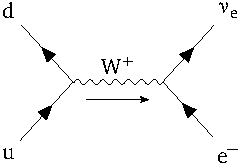
\includegraphics{ec}
    \caption{%
        Electron capture, leading order contribution. Time goes upwards.
    }
    \label{fig:ec}
\end{figure}

\begin{figure}
    \centering
    \includegraphics{co57}
    \caption{%
        Decay scheme of $^{57}\mathrm{Co}$ into $^{57}\mathrm{Fe}$. Cobalt from
        the source undergoes electron capture (EC) with a very long halftime.
        The transition between to the groundstate (thick) is the Mößbauer
        energy level we are interested in.
        %
        Figure adapted from
        \textcite[Fig.~4.8]{Schatz/Nukleare_Festkoerperphysik}.
    }
    \label{fig:co57}
\end{figure}

The emission lines are not perfectly sharp. This limits the chance of
absorption by the same kind of nucleus. The broadening effects are the
following:

\begin{description}
    \item[Natural width]
        The lifetime $\tau$ of every metastable state is limited. If it were
        not, one would not observe the transition. Together with the
        energy-time-uncertainty this directly leads to a line width of
        \[
            \Gamma = \frac\hbar\tau \,.
        \]
        Our line of interest, the \SI{14.4}{\kilo\electronvolt}-line has a
        lifetime of \SI{141}{\nano\second} and therefore a width of $\Gamma =
        \SI{4.7e-9}{\electronvolt}$. Compared to energy of the photons
        themselves, this is a relative width of \num{3.3e-13} which is very
        small compared to the other effects.
        \parencite[42]{Schatz/Nukleare_Festkoerperphysik}

    \item[Doppler effect]
        A relative motion between source and target will lead to a Doppler
        shift. The Lorentz transformation connecting the two systems boosts the
        photon's energy. If the source particles are subject to thermal
        motions, the spectrum will be broadened. At room temperature the shifts
        in energy are around \SI{10e-2}{\electronvolt}
        \parencite[43]{Schatz/Nukleare_Festkoerperphysik}, depending on the
        angle of motion and emission.

        The natural line width could be ignored when the Doppler effect is
        present.

    \item[Recoil]
        The photon carries momentum $\hbar k$. In the center of mass frame of
        the emitting nucleus, the nucleus will take the recoil $- \hbar k$. The
        energy of the nucleus then is $(\hbar k)^2/2 M$, where $M$ is the mass
        of nucleus. This energy is subtracted from the photon; the photon has a
        reduced frequency when emitted from a free nucleus.
\end{description}

Taking all those effects together, it becomes unlikely that the photons emitted
by a gas of decaying cobalt will be absorbed by a gas of iron, ignoring that it
might be impractical to realize this situation. The issue of the recoil can be
reduced by embedding the nuclei of interest into a solid. The lattice will
absorb the excess momentum and due to its practically infinite mass (\num{e23}
larger), there will be no recoil velocity and therefore no energy shift in the
photon.

\section{Debye-Waller Factor}

Although there is no energy shift caused by recoil, the energy is still shifted
due to thermal motion of the atoms. Even at $T = \SI{0}{\kelvin}$, there will
be a shift because of zero-point energy. To get a measure of how temperature,
$\gammaup$-energy and mass of the lattice influence the emission, one can find
the Debye-Waller factor, which is the ratio of the unshifted spectrum to the
real one. For temperatures below the material specific Debye
temperature~$\Theta$ the factor is given by
\[
    f_\text{D} (T, E_\gammaup, M)
    = \exp \del{
        - \frac{3E_\gammaup^2}{4Mc^2k_\text{B}\Theta}
        \sbr{1 + \frac{2\piup^2}3 \del{\frac T\Theta}^2}
    } \,,
\]
analogue to the expression given by
\textcite[42]{Schatz/Nukleare_Festkoerperphysik}.

For iron, the Debye temperature is $\Theta = \SI{470}{\kelvin}$
\parencite[Tab.~6.1]{Hunklinger/Festkoerperphysik}, so we are well below this
in our experiment. Together with $E_\gammaup = \SI{14.4}{\kilo\electronvolt}$,
the iron mass $M = \SI{<< iron_mass >>}{\kilogram}$ and assuming room
temperature ($T = \SI{<< room_temperature >>}{\kelvin}$), we see that the
fraction has the value \num{<< debye_1 >>}, the square bracket has the value
\num{<< debye_2 >>} which yields a total Debye-Waller factor of \num{<< debye_3
>>} for our experimental situation.

\section{Magnetic hyperfine structure}

The angular momentum $l$ and the spin $s$ of the nucleus couple to a combined
spin $j$. The component along the quantization axis, $m_j$, takes values
between $-j$ and $j$. The various states organize themselves into the
irreducible representations of $\SU(2)$, the multiplets with spin $j$ and
$(2j+1)$ states each. The different multiplets have different energies, the
energies within the same multiplet are degenerate, see left part of
Figure~\ref{fig:M1}. Breaking the $\SU(2)$ symmetry of the spins give the
nuclear analogue of the Zeeman effect. This is done with an external magnetic
field by the interaction term $- \vec\mu \cdot \vec B$. The degeneracy is
broken and each multiplet is split up into equidistant levels, see the right
part of said figure.

The magnetic moment $\vec \mu$ is coupled to the spin via the nuclear magneton
$\mu_\text N$ or the gyromagnetic ratio $\gamma$,
\[
    \mu = \underbrace{g \frac{\mu_\text N}{\hbar}}_{\gamma} \hbar j \,.
\]
Choosing the quantization axis along the external magnetic field $\vec B$ will
simplify the interaction $- \vec \mu \cdot \vec B$ to $- g \mu_\text N m_j$.
The $m_j$ are (half-)integers and therefore equidistant. This makes the energy
levels equidistant within a multiplet.

\begin{figure}
    \centering
    \includegraphics{M1}
    \caption{%
        Hyperfine structure of the \SI{14.4}{\kilo\electronvolt}-M1-line in
        $^{57}\mathrm{Fe}$, our Mößbauer transition.
        Figure adapted from
        \textcite[Fig.~4.22]{Schatz/Nukleare_Festkoerperphysik}.
    }
    \label{fig:M1}
\end{figure}

Both source and target are embedded into a solid, therefore there is
little thermal fluctuation and also very little recoil. This means that the
lines are rather sharp. Only the target is embedded into a magnetic field. The
source iron nuclei do not have the Zeeman splitting and therefore always emit a
pretty exact \SI{14.4}{\kilo\electronvolt} line. In order for the target in the
magnetic field to absorb this line, the energy needs to be adjusted.

By moving the source with a motor, one can leverage the Doppler shift to alter
the energy of the photon. As this velocity is controlled, one can effectively
measure the energy shifts and therefore the hyperfine structure in the iron
target. We are interested in the deviation from $\hbar \omega_0 =
\SI{14.4}{\kilo\electronvolt}$ and want to extract the magnetic moment of the
groundstate and the exited state.

The needed relation between Doppler velocity $v$ and the magnetic moments
$\mu$, $\mu'$ is
\[
    v = - \frac{c B}{\hbar \omega_0}
    \sbr{\frac{\mu'}{j'} m_j' - \frac{\mu}{j} m_j}
    \,,
\]
where the primed quantities are the exited state
\parencite[(4.42)]{Schatz/Nukleare_Festkoerperphysik}. Expressing the magnetic
moments in terms of the nuclear magneton, we see the relation between the Landé
factors more clearly:
\begin{equation}
    \label{eq:velocity}
    v = - \frac{c B \mu_\text N}{\hbar \omega_0} \sbr{g' m_j' - g m_j} \,.
\end{equation}
Inside the solid, the magnetic flux density is \SI{<< B >>}{\tesla}. All other
quantities are known,
the prefactor has the value \SI{<< v_prefactor >>}{\meter\per\second}. As $g$
and $m_j$ are of the order of magnitude one, the experimental setup with
$v_\text{max} = \SI{0.006}{\meter\per\second}$ will be sensible.

The selection rule for magnetic dipole radiation (M1) is $(m_j - m_j') \in \{
-1, 0, 1 \}$. Therefore we expect to see six velocities with high absorption.

\section{Isomeric shift and quadrupole moment}

The iron nuclei in the source and target are embedded into a solid. This means
that each nucleus is surrounded by a lot of other charged particles which
create a non-constant electric field. The nucleus is not a point charge,
therefore it does interact with the electric potential beyond a monopole
interaction.

We assume that the electric potential that is created outside of the nucleus
does not vary too much across the volume of the nucleus. Then we can expand the
electric potential around the nucleus like
\[
    \Phi(\vec r) = \Phi_0 + \pd{\Phi}{x^i} x^i
    + \frac12 \frac{\partial^2 \Phi}{\partial x^i \partial x^j} x^i x^j +
    \mathrm O(x^3) \,,
\]
where we have used Einstein's summation convention
\parencite[(3.19)]{Schatz/Nukleare_Festkoerperphysik}. We can identify three
terms:

\begin{description}
    \item[Constant]
        The constant term is the monopole interaction, it just gives rise to a
        common shift in the energies and is not relevant for our experiment as
        we can only observe the difference in energy levels, i.e.\ the photon
        energy.

    \item[Linear]
        The gradient is a dipole interaction. Quantum mechanics enforces the
        nuclear states to be parity eigenstates, therefore the expectation
        value of the dipole moment is zero. The linear term does not create any
        shift in the energy.

    \item[Quadratic]
        The Hessian gives rise to an electric quadrupole interaction and the
        isomeric shift. We will need to further analyze the Hessian.
\end{description}

The shift in energy by each of those terms is given by an appropriate
integration against the charge density of the nucleus. For the quadratic term
we have
\[
    E^{(2)} = \frac 12 \frac{\partial^2 \Phi}{\partial x^i \partial x^j}
    \int \dif^3 r \, \rho(\vec r) \, x^i x^j \,.
\]
Since the Hessian is a real symmetric matrix, it can be diagonalized by an
orthogonal transformation. Let the eigenvalues of the Hessian be $\lambda_i$,
then we can split up the electric energy like follows:
\begin{align*}
    E^{(2)}
    &= \frac12 \sum_i \lambda_i \int \dif^3 r \, \rho(\vec r) \, x_i^2 \\
    &= \frac16 \sum_i \lambda_i \int \dif^3 r \, \rho(\vec r) \, r^2
    + \frac12 \sum_i \lambda_i \int \dif^3 r \, \rho(\vec r) \sbr{x_i^2 -
    \frac{r^2}3} \,.
\end{align*}
The electric potential also obeys the Poisson equation, therefore we also have
\[
    \laplace \Phi = \sum_i \lambda_i = \frac{e}{\varepsilon_0} |\psi(0)|^2 \,,
\]
i.e.\ the charge density at the origin by the electron wavefunctions is the
trace of the Hessian. The first summand in the above splitting is the isomeric
term and we can rewrite it as
\[
    E_\text I := \frac16 \frac{e}{\varepsilon_0} |\psi(0)|^2
    \int \dif^3 r \, \rho(\vec r) \, r^2 \,.
\]
The integral over the charge density with $r^2$ is the second moment of the
charge distribution and therefore proportional to $\bracket{r^2}$, the
expectation value of the squared radius. The proper normalization includes
$1/Ze$.

We see that the isomeric term depends on the shape of the nucleus but does not
lead to any splitting depending on $m_j$ like we saw with an external magnetic
field.
The energy difference can be expressed as a Doppler velocity
\[
    v = \frac{Z e^2 c}{6 \varepsilon_0 \hbar \omega_0}
    \del{|\psi_\text T(0)|^2 - |\psi_\text S(0)|^2}
    \del{\bracket{r^2_\text{e}} - \bracket{r^2_\text{g}}} \,,
\]
as given by \textcite[(4.31)]{Schatz/Nukleare_Festkoerperphysik}. If the iron
nuclei in source (S) and target (T) are embedded into different crystals, then
$|\psi(0)|^2$ will be different there. We also need the mean squared radius of
the excited (e) and ground (g) state to differ in order for this effect to be
picked up. In our experiment we will see this as a common shift independent of
$m_j$.

\parencite[33, 34]{Schatz/Nukleare_Festkoerperphysik}

\chapter{Experimental setup and measurement}

\section{Setup}

%TODO better chapter title

The $^{57}\mathrm{Co}$ source is located in a shielding led box. The
$\gammaup$-rays escape through an opening in the target's direction. The
absorber is a thin $^{57}\mathrm{Fe}$ plate attached to a motor, which allows
us to move it with tunable but constant velocity over a distance of \SI{25.1 +-
0.2}{\milli\meter} unto the source and away from it. Behind the absorber there
is a proportional detector. Its signal is fed into an amplifier and then into a
single channel analyser (\textsc{sca}) compare to Figure~\ref{fig:electronics}.
After that the signals are counted in two counters ($n_\text{RL}$ and
$n_\text{LR}$) depending on the moving direction of the absorber. The direction
is given by the motor steering, as well as the total run number. The timer
gives a signal every \SI{10}{\milli\second} to another \textsc{sca}, which
leads the signal to the two counters $t_\text{RL}$ and $t_\text{LR}$
respectively, also depending on the moving direction.


\begin{figure}
    \centering
    \includegraphics{electronics}
    \caption{%
        Principal scheme of the electronic setup.
    }
    \label{fig:electronics}
\end{figure}


First we have to find the measurement's energy window with an oscilloscope to only
count $\SI{14.4}{\kilo\electronvolt}$ incidents and to reduce noise. After that
we reset all counters and start the measurement by pressing the start button on
the motor steering. The counting begins at the left turning point and will also
stop at this point to make sure there are as many \textsc{lr} runs as
\textsc{rl}. 

\section{Measurement}

We start the first measurement by resetting all the counters and starting the
motor controller. On the next full left swing of the absorber, the gates are
opened and we see the counters work.

After a couple minutes, the number of events on both sides ($\nLR$ and $\nRL$)
are over \num{7000}. We instruct the motor controller to stop. Then at at the
next full left swing, the measurement is stopped. The number of runs $N$, the
motor setting, the times $\tLR$ and $\tRL$ as well as the number of events
$\nLR$ and $\nRL$ are read off by us.

Then we change the motor setting by four ticks on the scale and let it run
again.

\section{Analysis}

\subsection{Velocity of target}

First we have to compute the actual velocity of the target. In each measurement
we have $N$ runs back and forth. The displacement for one direction (half a
run) is $s = \SI{<< length_mm >>}{\milli\meter}$. The total time spend going
from left to right is $\tLR$, so we can compute the velocity with
\[
    \vLR = \frac{s N}{\tLR}
    \qquad\text{and}
    \vRL = \frac{s N}{\tRL}
    \,.
\]

We were warned that the relation between the motor setting and the actual speed
might not be linear. Therefore we have checked this, see Figure~\ref{fig:motor}
for a graphical representation of the data. It is linear but the velocities in
left--right and right--left direction are not the same. This is not a problem
as we use the velocity and not the motor setting for the analysis.

\begin{figure}
    \centering
    \includegraphics{motor}
    \caption{%
        Relation of motor setting (units on the control potentiometer) and the
        actual speed.
    }
    \label{fig:motor}
\end{figure}

For each measurement, we compute the count rate simply with $\rateLR = \nLR /
\tLR$ (and similar to right--left). The count rates are shown versus the
velocity in Figure~\ref{fig:count_rate}. There we can see the transmission
spectrum. The background of around \SI{60}{\per\second} is the transmission of
the lines to the detectors. We see six distinct dips in the transmission, those
are the resonance frequencies. Keeping in mind that the photon energy is $\hbar
\omega_0 (1 + v/c)$ and $v \ll c$ in our experiment, the lines are remarkably
sharp.

\begin{figure}
    \centering
    \includegraphics{count_rate}
    \caption{%
        Count rate versus velocity. Also included is a fitted sum of six
        Lorentzian curves and a constant offset.
    }
    \label{fig:count_rate}
\end{figure}

We fit a sum of six Lorentzian curves and a constant offset to the data. In
order to make this $6 \times 3 + 1 = 19$ parameter system stable, we carefully
tune the initial parameters of the least-squares-algorithm. Table~\ref{tab:fit}
holds our fit parameters for the Lorentzian curves, the constant offset is
\SI{<< fit_offset >>}{\per\second}. The error estimates are the square roots of the
diagonal of the covariance matrix.

\begin{table}
    \centering
    \begin{tabular}{SSS}
        \toprule
        {$\mu / \si{\milli\meter\per\second}$}
        & {$\Gamma / \si{\milli\meter\per\second}$}
        & {$I / \si{\milli\meter\per\second\squared}$} \\
        \midrule
        %< for row in fit_param >%
        << ' & '.join(row) >> \\
        %< endfor >%
        \bottomrule
    \end{tabular}
    \caption{%
        Fit parameters and errors for the Lorentz dips. We have the mean $\mu$,
        the width $\Gamma$ and the integral $I$.
    }
    \label{tab:fit}
\end{table}

\end{document}

% vim: spell spelllang=en tw=79
